%\newcommand{\CLASSINPUTbaselinestretch}{1.0} % baselinestretch
%\newcommand{\CLASSINPUTinnersidemargin}{1in} % inner side margin
%\newcommand{\CLASSINPUToutersidemargin}{1in} % outer side margin
%\newcommand{\CLASSINPUTtoptextmargin}{1in}   % top text margin
%\newcommand{\CLASSINPUTbottomtextmargin}{1in}% bottom text margin

\documentclass[journal,a4paper]{IEEEtran}


\usepackage[pdftex]{graphicx}  
\usepackage[cmex10]{amsmath}
\usepackage[dutch]{babel}

\usepackage{float}
\usepackage{caption}
\usepackage[caption = false,subrefformat=parens,labelformat=parens]{subfig}
\usepackage{amsmath}
\usepackage{epstopdf}
\usepackage{textcomp}
\usepackage{gensymb}
\usepackage[titlenumbered,algoruled, linesnumbered]{algorithm2e}
\usepackage{algpseudocode}
\usepackage{booktabs}
\usepackage[T1]{fontenc}
\usepackage[utf8]{inputenc}


\newcommand\MYhyperrefoptions{bookmarks=true,bookmarksnumbered=true,
pdfpagemode={UseOutlines},plainpages=false,pdfpagelabels=true,
colorlinks=true,linkcolor={black},citecolor={black},pagecolor={black},
urlcolor={black},
pdftitle={Flip the virus:\\ A gametheoretic approach to cybersecurity},
pdfauthor={Sophie Marien}}

\begin{document}

\title{Flip the virus:\\ A gametheoretic approach to cybersecurity}
\author{Sophie Marien}
\maketitle

\IEEEcompsoctitleabstractindextext{%
\begin{abstract}
Recently the attacks on Belgacom and other high profile targeted attacks shows us that even
the most secure companies can still be compromised. It also shows that these attacks are
not immediately detected. FlipIt is a framework that can model these stealthy takeovers and is
proposed by a group of researchers at RSA. It is a 2-players game composed of a single attacker,
a single defender and a single shared resource. These players will try to gain control over the
shared resource and they do this in a stealthy way. In this paper we try to adapt FlipIt in a
way that we can use it to model the game of defending a company network that is attacked by a virus. The FlipIt formulas are adapted for this virus propagation. Through analytic results we can provide
useful information for the defender to defend his network.
\end{abstract}
}

\IEEEdisplaynotcompsoctitleabstractindextext
\IEEEpeerreviewmaketitle


\section{Inleiding}
\label{sec:inleiding}
\IEEEPARstart{I}{n this era} where digitalization becomes prominent in every aspect of our lives, where technology is growing fast and where businesses are always under attack, security becomes an issue of increasing complexity. Without security, there is no protection to keep somebody out of a system. It is the same as leaving the door of your house wide open for everyone to come in. Why is it so important to keep a system secure?  \\

Businesses can have confidential information on clients. Through data leakage, confidential information can be lost and possibly used by the competitor. Businesses wants to meet their service-level agreements. They will protect themselves against disruption that can be caused by DOSS attacks. Ultimately, system and network security helps protecting a business's reputation, which is one of its most important assets. %\todo{waarom?  :  lekken van informatie: je hebt info over klanten en moet hun privacy beschermen, je eigen data is geld waard voor concurrenten, DOSS attacks: je will je service-level agreements kunnen nakomen, ..} \\
 A hacker will be a person that seeks exploits or weaknesses in a system or network in order to gain access.  Many of those attacks have a different cause. Some of the attacks by a hacker can be benign, others can be harmful. There are various ways to break into a system. Viruses, worms, spyware and other malware are the number two of the top external threats that a business faces, according to the security report kaspersky 2014 \cite{kaspersky} (number one is Spam). Furthermore these kind of threats also causes the greatest percentage in loss of data. These threats will infect the network by means of a virus that will propagate through the network.  Most of the attacks are Advanced Persistent Threats (APT). \\
 
An APT is a targeted cyber attack that targets organisations in a stealthy way and stays undetected for a long period. This makes it so hard to protect against an APT. Bruce Schneier describes an APT as something different and stronger than a conventional hacker: ''\textit{A conventional hacker or criminal isn't interested in any particular target. He wants a thousand credit card numbers for fraud, or to break into an account and turn it into a zombie, or whatever. Security against this sort of attacker is relative; as long as you're more secure than almost everyone else, the attackers will go after other people, not you. An APT is different; it's an attacker who - for whatever reason - wants to attack you. Against this sort of attacker, the absolute level of your security is what's important. It doesn't matter how secure you are compared to your peers; all that matters is whether you're secure enough to keep him out}'' - Bruce Schneier: APT is a Useful Buzzword.\\


\section{Stealthy takeover model}
Since it is so difficult to protect a system or a network against APT, researcher have been looking for effective ways to predict in advance which defence strategy might be the better one. 
Game theory is gaining more and more interest as an effective technique to  model and study Cyber Security. Game theory analyses the security problem as a game where the players are an attacker and a defender of a system, and where both players have to make decisions. In particular, both players will aim for the strategy that results in a maximal benefit for them.  Researchers at RSA made a game theoretic framework to model targeted attacks. They study the specific scenario where a system or network is repeatedly taken over completely by an attacker and this attack is not immediately detected by the defender of the system or network. In game theory, such a game is known as ''FlipIt'' \cite{FlipIt}. This is a two players game where the attacker and the defender are competing to get control over a shared resource. Both players do not know who is currently in control of the resource until they move. In FlipIt every move gives them immediately control over the resource. But what if the attacker moves and it takes a while before the attacker gets full control over the resource? FlipIt does not take into account that a move may not be instantaneous, but has a certain delay. Consider for example a network with different nodes ( laptops, datacenters) as a resource. The attacker drops a virus on one of the nodes and then wait till this virus infects the whole network. The attacker will only be in control of the resource once the whole network is infected. \\


\begin{figure}[hbtp]
\caption{FlipIt game with a periodic strategy. The defender plays with a period of deltaA = .. The attacker plays with a period $\delta_{A}$ }
\centering
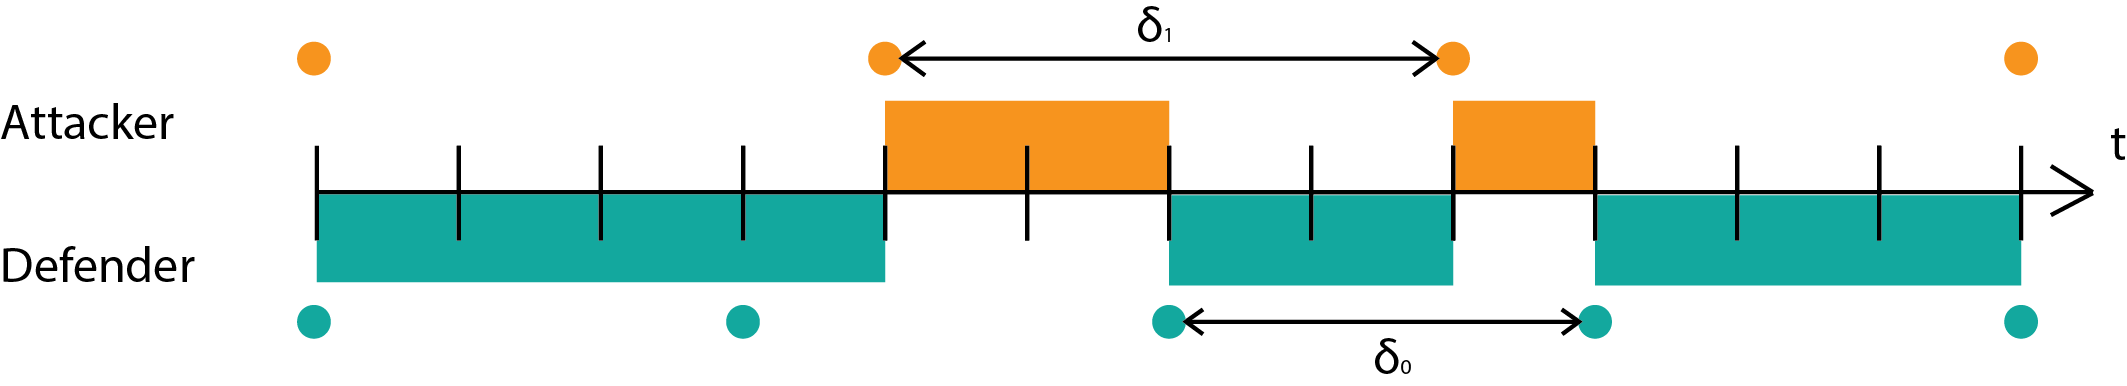
\includegraphics[scale=0.5]{../../doc/template/Images/DefFlipIt.png}
\end{figure}

\section{FlipIt with virus propagation}
A FlipIt game consists of a single resource. To represent the security problem, the game now defines its single resource as a computer network with multiple
nodes. One of the players, the defender, will try to defend his network. The defender
will do this by flipping all the nodes of the network (i.e. the entire resource) in every move he plays. The
attacker, the other player, will try to infect all the nodes in the network. The attacker
will do this by flipping the node in the graph that can infect all the nodes in the
shortest time possible. After dropping a virus on the first node, it takes a while for the virus to infect the entire network. However, since the original FlipIt game works with a single resource that is always flipped entirely, the assumption is made that the attacker is considered to have gained the control over the resource only when all the nodes of the network have been infected, i.e. the entire resource has been flipped.\\

After dropping a virus on the first resource, it takes a while for the virus to infect
the entire network. The time that it takes for the virus to infect every node will be
denoted as parameter d. If we want to measure how long it takes for the virus to
infect all the nodes in the network, we have to calculate the shortest path from the
first infected node to the farthest node. This can be measured by a method that we
will explain in section []. Assume that an attacker attacks at time t, then only at time t + d he gains control over the entire network. If the defender flips the network before the period d has elapsed (so, somewhere between t and t+ d), then the attacker will never gain control over the entire network. Using this parameter d, a FlipIt game with virus propagation
can be modelled. \\

We start by formalizing the non-adaptive continuous basic FlipIt game where players use a periodic strategy with a random phase. his choice is motivated by the assumption that in the practical situation of most organisations, the defence strategy is to periodically defend the network. This corresponds to a periodic defender strategy.  To simplify the analysis in a first time, a periodic attacker strategy is assumed as well. Further research can investigate the effect of relaxing this assumption. \\

Next we split the formalisation for the benefit formula for a FlipIt game with virus propagation in two cases. First the benefit formula is derived for the basis case and then it is calculated for the case with a virus propagation. The first case is where the defender plays at least as fast as the attacker, the second case is where the attacker plays at least as fast as the defender. This subdivision is also used in the FlipIt paper. \\

 A Periodic strategy is a non-adaptive renewal strategy where the time intervals between consecutive moves are a fixed period, denoted by $\delta$. Moreover it has a random phase, that is chosen uniformly and random in the interval $[0,\delta]$ for the first move. The average rate of play of a player is denoted by $\alpha_{i} = \dfrac{1}{\delta_{i}}$. \\
~~\\


\subsection*{\textbf{Case 1:} $\delta_{D} \leq \delta_{A} $ (The defender plays at least as fast as the attacker.) }

Let $r = \dfrac{\delta_{D}}{ \delta_{A} }$. The intervals between two consecutive defender's moves have length $\delta_{D}$. Consider a given defender move interval. The probability over the attacker's phase selection that the attacker moves in this interval is r. Given that the attacker moves within the interval, he moves exactly once within the interval (since $\delta_{D} \leq \delta_{A} $) and his move is distributed uniformly at random. \\

The expected period of attacker control within the interval would be r/2, without considering the delay by a virus. Therefore the benefit without this virus can be expressed as follows:
\begin{equation}\label{first}
\beta_{D}(\alpha_{D},\alpha_{A}) =1 -  \dfrac {r} {2} - k_{D} \alpha_{D} = 1 - \dfrac {\delta_{D}} {2\delta_{A}} - k_{D} \alpha_{D} 
\end{equation}
\begin{equation}\label{first}
\beta_{A}(\alpha_{D},\alpha_{A}) =\dfrac {r} {2} - k_{A} \alpha_{A} = \dfrac {\delta_{D}} {2\delta_{A}} - k_{A} \alpha_{A}  
\end{equation}\\

However, because of the delay caused by a virus, the maximal time of control is reduced to $\delta_{D}-d$. There is a probability of \textit{r} that the attacker will move in the interval of the defender. The attacker has to play soon enough to gain control, meaning that the attacker has to play during the period of $\delta_{D}-d$ during the interval of the defender. There is $\dfrac{\delta_{D}-d}{\delta_{D}}$ probability that the attacker will move soon enough which gives the attacker a gain of $\dfrac{\delta_{D}-d}{2}$. If the attacker moves after the period of $\delta_{D}-d$, the gain of the attacker will be zero. The average gain rate of the attacker can be expressed as follows if we look at one interval of the defender:
\begin{equation}\label{first}
\beta_{A}(\alpha_{D},\alpha_{A}) = \dfrac {1}{\delta_{D}} [ \dfrac{\delta_{D}}{\delta_{A}} \cdot \dfrac{\delta_{D}-d}{\delta_{D}} \cdot \dfrac{\delta_{D}-d}{2} + \dfrac{\delta_{D}}{\delta_{A}} \cdot \dfrac{d}{\delta_{D}} \cdot 0 ]
\end{equation}

To complete the formula to derive the benefit function, the cost of moving is added. In the second formula we can see the formula of the original FlipIt game.
\begin{equation}\label{first}
\beta_{A}(\alpha_{D},\alpha_{A}) = \dfrac { (\delta_{D}-d) ^{2}} {2 \cdot \delta_{D}  \delta_{A}} - k_{A} \alpha_{A}
\end{equation}
\begin{equation}\label{first}
\beta_{A}(\alpha_{D},\alpha_{A}) = \dfrac { \delta_{D}} {2 \cdot \delta_{A}} - k_{A} \alpha_{A} + \dfrac{d}{\delta_{A}} + \dfrac{d^{2}}{2 \cdot \delta_{A} \delta_{D}}
\end{equation}
 
 The benefit of the defender is expressed as follows:
 \begin{equation}\label{first}
\beta_{D}(\alpha_{D},\alpha_{A}) = 1 - \dfrac { (\delta_{D}-d) ^{2}} {2 \cdot \delta_{D}  \delta_{A}} - k_{D} \alpha_{D}
\end{equation}
~~\\



\subsection*{\textbf{Case 2:} $\delta_{A} \leq \delta_{D} $ (The attacker plays at least as fast as the defender.) }

First let $r = \dfrac{\delta_{D}}{ \delta_{A} }$. The intervals between two consecutive attacker's moves have length $\delta_{A}$. Consider a given attackers move interval. The probability over the attacker's phase selection that the defender moves in this interval is $\dfrac{\delta_{D}}{ \delta_{A} } = (1/r)$. Given that the defender moves within the interval, he moves exactly once within the interval (since$\delta_{A} \leq \delta_{D} $) and his move is distributed uniformly at random. \\

A similar analysis as in case 1 for a FlipIt game without virus propagation yields the following benefits:
\begin{equation}\label{first}
\beta_{D}(\alpha_{D},\alpha_{A}) = \dfrac {1} {2r} - k_{D} \alpha_{D} = \dfrac {\delta_{A}} {2\delta_{D}} - k_{D} \alpha_{D} 
\end{equation}
\begin{equation}\label{first}
\beta_{A}(\alpha_{D},\alpha_{A}) =1 - \dfrac {1} {2r} - k_{A} \alpha_{A} = 1- \dfrac {\delta_{A}} {2\delta_{D}} - k_{A} \alpha_{A}  
\end{equation}\\


For the case with a virus we consider two cases, Case a and Case b, to compute the benefit of both players.  \\


\subsubsection*{\textbf{Case a:} $d + \delta_{A} \leq \delta_{D}$}

Let $d + \delta_{A} \leq \delta_{D}$. If $d + \delta_{A}$  is a timespan for the attacker, the defender will never move twice in this timespan.  $\dfrac{delta_{A}}{\delta_{D}}$ the defender will move during the interval of the attacker. When this happens the defender will end with being in control at the end of the interval. In the next interval the attacker will move in the beginning but will not gain control after the delay of \textit{d}. This means that if the defender moved in the interval prior to this one, the delay is the minimum gain of the defender. To calculate the gain rate of the defender we don't look at one interval of the defender. We know that if the defender moves within the interval of the defender, he will receive a minimum of $\dfrac{\delta_{A}}{2}$ gain. In the next interval the defender will receive a gain of $d$. 

This means that every time the defender plays, he will get a gain of $\dfrac{\delta_{A}}{2}$ and the next interval will always receive a gain of $d$. To derive the benefit formula for the defender we can calculate the probability that the defender will move during an interval of the attacker and multiply it by the gain rate of the defender plus the gain rate that it will give to the next interval. 
This yields in the following formula:
\begin{equation}\label{first}
\beta_{D}(\alpha_{D},\alpha_{A}) = \dfrac{\delta{A}}{\delta_{D}} \cdot \dfrac{(d+\dfrac{\delta_{A}}{2})}{\delta_{A}} - k_{D} \alpha_{D} 
\end{equation}
\begin{equation}\label{first}
\beta_{D}(\alpha_{D},\alpha_{A}) = \dfrac{\delta{A}}{2\delta_{D}} + \dfrac{d}{\delta_{D}} - k_{D} \alpha_{D} 
\end{equation}\\

The benefit for the attacker will be as follows:
\begin{equation}\label{first}
\beta_{A}(\alpha_{D},\alpha_{A}) = 1 -\dfrac{\delta{A}}{2\delta_{D}} - \dfrac{d}{\delta_{D}} - k_{A} \alpha_{A} 
\end{equation}\\

\begin{figure}[hbtp]
\caption{Case 2 where d + deltaA < deltaD}
\centering
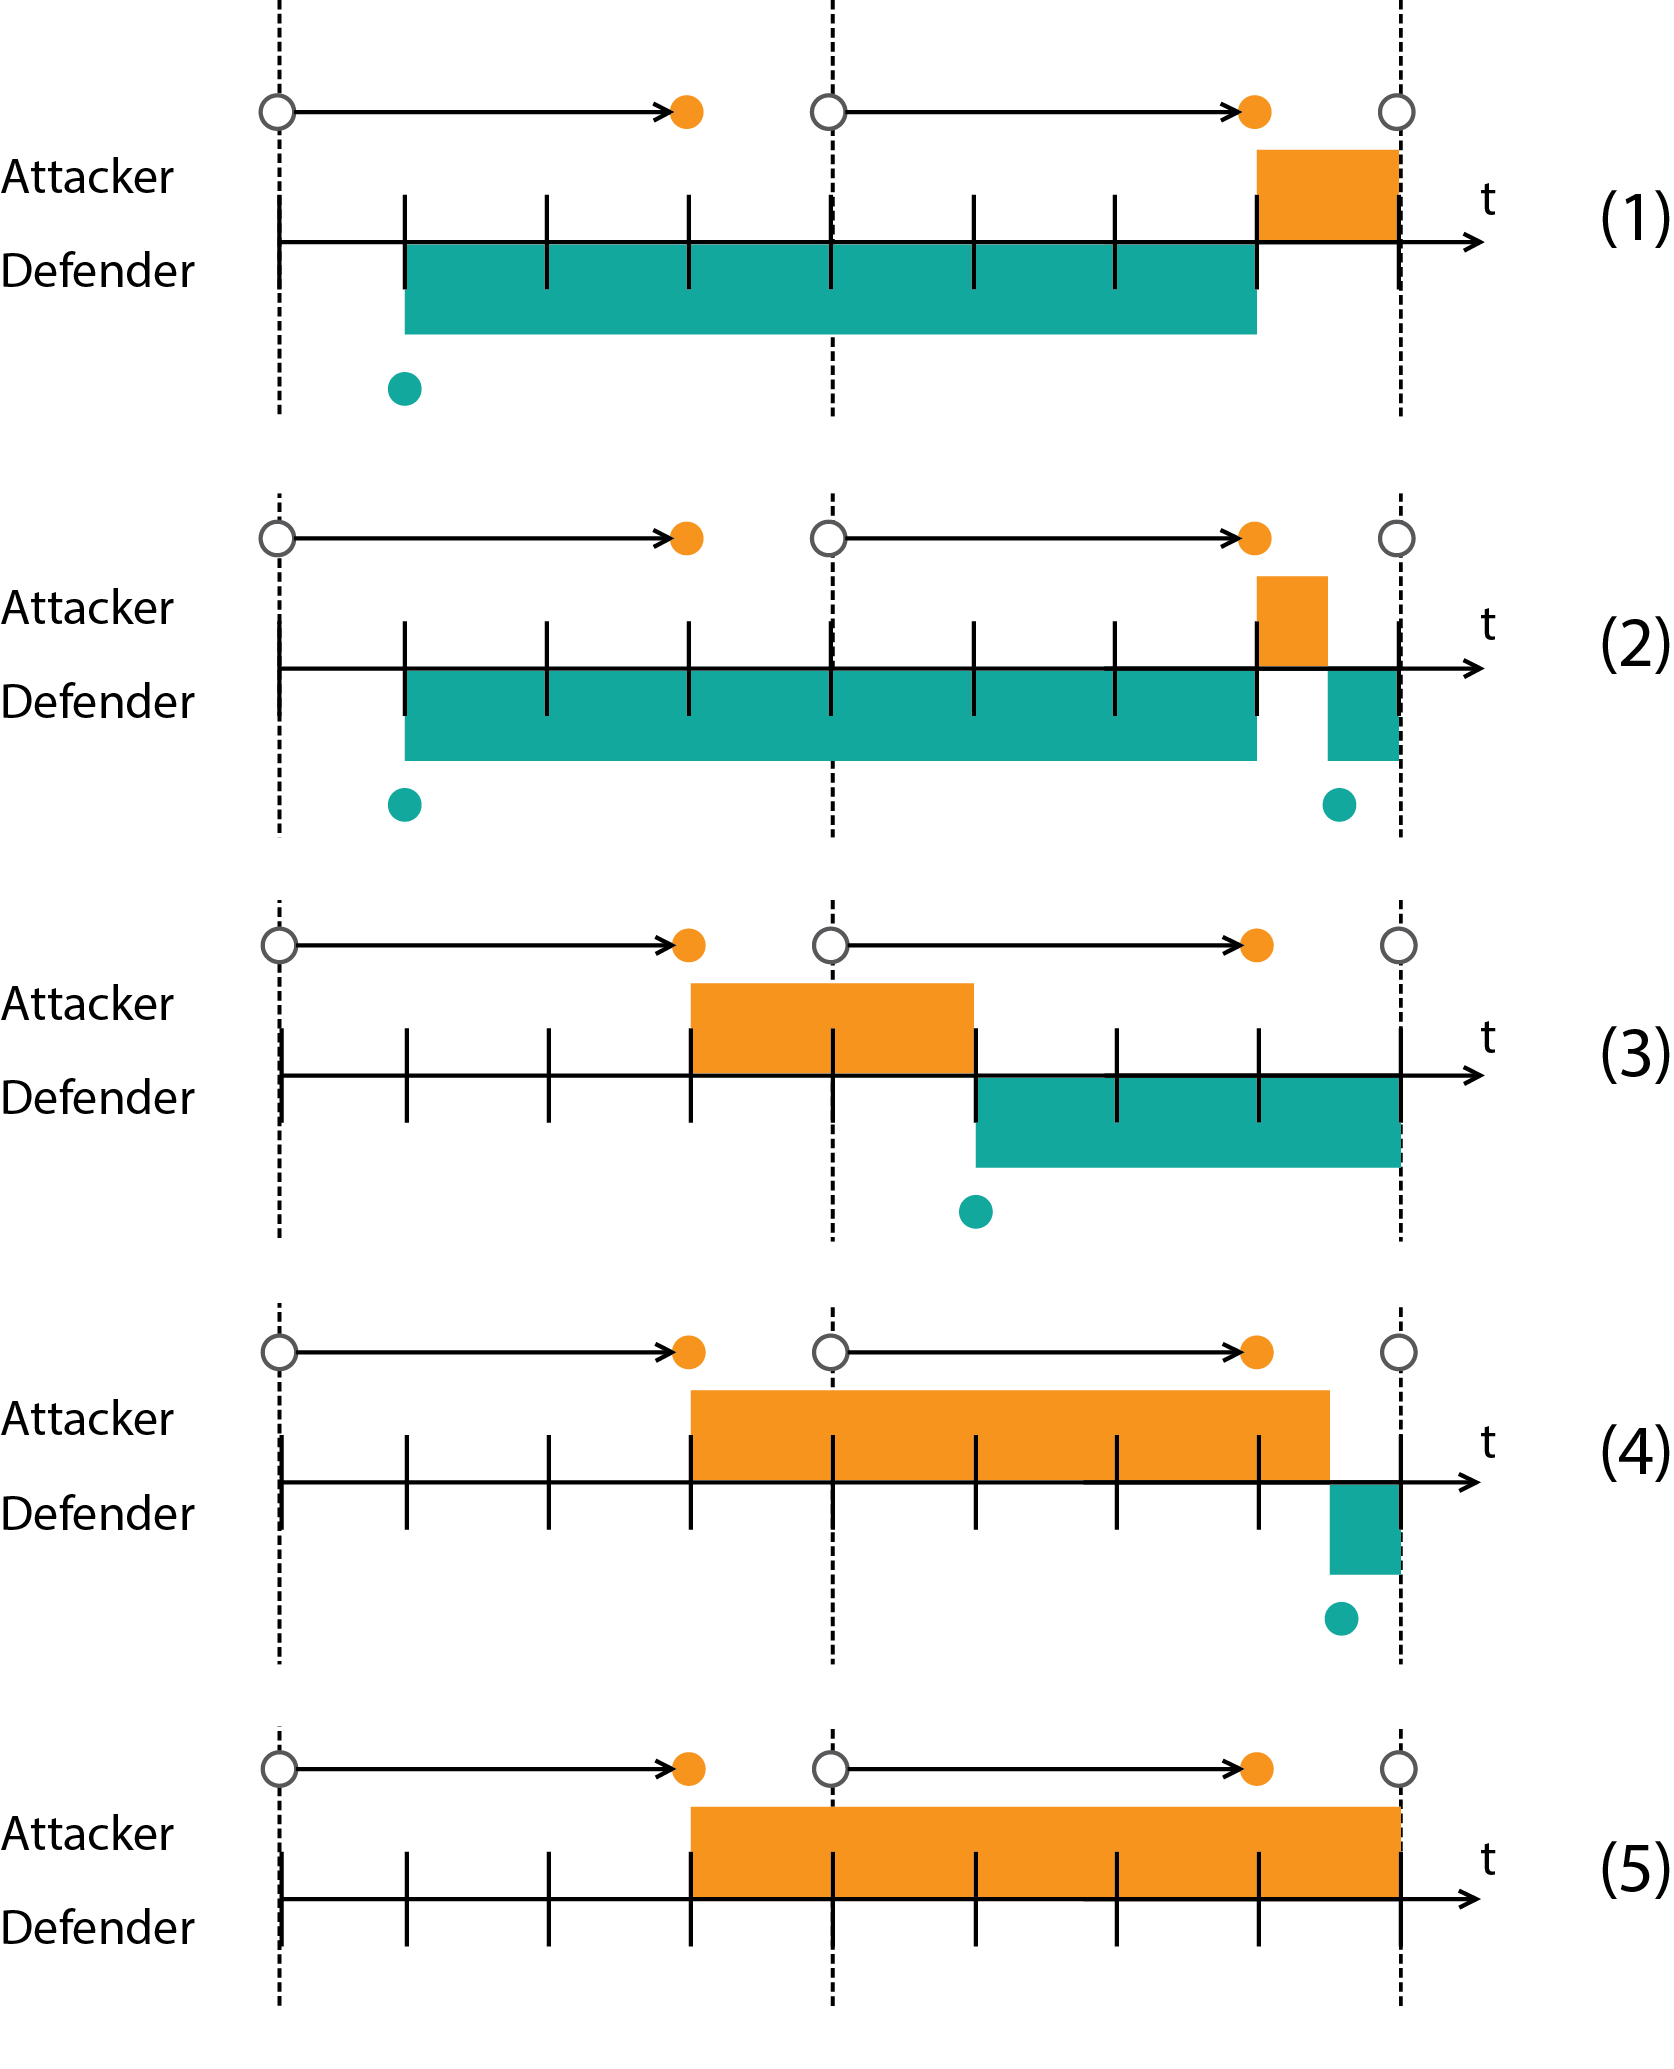
\includegraphics[scale=0.7]{../../doc/template/Images/FlipItCase2.png}
\end{figure}


It is crucial that the $d + \delta_{1}$ is not greater than $ \delta_{0}$. If it is greater that means that the defender can move during a delay after an interval of the attacker where the defender already has moved. If we calculate the benefit formula in the same manner, to much gain is added. Namely the overlap during the delay.

\subsubsection*{\textbf{Case b:} $d + \delta_{1} > \delta_{D}$}


\bibliographystyle{IEEEtran}
\bibliography{IEEEabrv,references}

\end{document}